%!TEX encoding = UTF-8 Unicode
% !TeX spellcheck = en_GB
%%%%%%%%%%%%%%%%%%%%%%%%%%%%%%%%%%%%%%
\chapter{ Virtual two-loop calculation of  $Zh$ production via gluon fusion}\label{chap:hz}
%%%%%%%%%%%%%%%%%%%%%%%%%%%%%%%%%%%%%%
\par  Higgs couplings to the weak vector bosons are approaching the precision level. For their measurements, both VBF and $Vh$ channels are needed. The associated Higgs production with the vector bosons is crucial for measuring the $VVh$ coupling amongst others, as discussed in~\autoref{vhproduction}. The most notable example emphasising the importance of this channel is the measurement of the Higgs decaying to beauty quarks~$h \rightarrow b \bar{b}$ by both ATLAS and CMS~\cite{Aaboud:2018zhk, Sirunyan:2018kst}. The statistical and systematic uncertainties coming from the experimental setup of the LHC will be eventually reduced in future runs due to higher integrated luminosity,  upgraded detectors and improved analysis techniques. There is an exigency to reduce theoretical uncertainties emerging from the perturbative calculations of cross-sections; to achieve that, one should include higher-order terms. As mentioned before, the $Wh$ channel has a much smaller theoretical uncertainties that $Zh$ due to the lack of gluon-fusion component in the former. This is due to the fact that the main source of uncertainties stems from the gluon fusion sub-process present in $Zh$. Higher-order corrections to the $gg \to Zh$ are essential for improving the theoretical modelling of this process. \\ 
It should be noted that the $Zh$ channel can receive contributions from new particles~\cite{Harlander:2013mla}, also as we shall see in~\autoref{chap:flav}; particularly at the large invariant-mass region where the gluon fusion contribution becomes more important, and the HTL approximation would typically fail. Therefore, a better understanding of the SM prediction of the $Zh$ gluon fusion channel is crucial for the SM precision measurements of Higgs production and testing NP in this channel.  \\ 
This chapter aims to demonstrate the use of the $\pt$--expansion technique, developed in ~\cite{Bonciani:2018omm} as an approach for computing the two-loop virtual corrections to $gg \to Zh$ analytically, including top quark mass effects. 
As has ben demonstrated in ref.~\cite{Bellafronte:2022jmo}, this method can be further upgraded with Pad\'e approximants and combined wit the HE expansion of~\cite{Davies:2020drs}. This allows to describe the whole phase space analytically.
\par This chapter is structured as follows: \autoref{chap6sec:GenNot} contains the general notation that is used for the gluon fusion production $Zh$ production calculation. Then in~\autoref{sec:ptexp}, the transverse momentum expansion method is discussed.  Calculation of the LO form-factors in the transverse momentum expansion is illustrated in~\autoref{sec:LOPtExp} as a proof of concept for this technique. The outline of the two-loop calculation is discussed in~\autoref{sec:quattro}. Finally, in~\autoref{sec:hzres}, the results of this calculation are shown with concluding remarks at the end.  This chapter is based on the work that my collaborators and I have published in~\cite{Alasfar:2021ppe}. 
%%%%%%%%%%%%%%%%%%%%%%%%%%%%%%%%%%%%%%%%%%%%%%%%%
\section{General notation \label{chap6sec:GenNot} }
\par The amplitude  $g^\mu_a(p_1)g^\nu_b(p_2)\to Z^\rho(p_3) h(p_4)$ can be written as
\begin{align}
	&&\amp=i \sqrt{2}\frac{\mz \Gfer \as(\mu_R)}{\pi}\delta_{ab}\epsilon^a_\mu(p_1)
	\epsilon^b_\nu(p_2)\epsilon_\rho(p_3)\hat{\amp}^{\mu\nu\rho}(p_1,p_2,p_3 ),\\
	&&\hat{\amp}^{\mu\nu\rho}(p_1,p_2,p_3 )=\sum_{i=1}^{6}
	\mathcal{P}_i^{\mu\nu\rho}(p_1,p_2,p_3 )
	\amp_i(\hat{s},\hat{t},\hat{u},\mt,\mh,\mz),
	\label{eq:amp}
\end{align}
where  $\mu_R$ is the renormalisation scale and
$\epsilon^a_\mu(p_1)\epsilon^b_\nu(p_2)\epsilon_\rho(p_3)$ are the
polarization vectors of the gluons and the $Z$ boson, respectively.  It is possible to decompose the amplitude into a maximum of six Lorentz structures encapsulated by the 
tensors $\mathcal{P}_i^{\mu\nu\rho}$. Due to the presence of the~$\gamma_5$, these projectors are
proportional to the Levi-Civita total anti-symmetric tensor
$\epsilon^{\alpha\beta\gamma\delta}$. One can choose to project the amplitude using a set of orthogonal basis, which is explicitly shown in~\autoref{app:uno}. 
By this choice one obtains unique form-factors corresponding to each projector
\begin{equation}
	\amp_i(\hat{s},\hat{t},\hat{u},\mt,\mh,\mz),
\end{equation}
that are multivariate complex functions of the
top quark ($\mt$), Higgs ($\mh$) and $Z$ ($\mz$) bosons masses, and of the partonic Mandelstam variables
\begin{equation}
	\hat{s}=(p_1+p_2)^2,~~ \hat{t}=(p_1+p_3)^2,~~ \hat{u}=(p_2+p_3)^2,
\end{equation}
where $\hat{s}+\hat{t}+\hat{u}=\mz^2+\mh^2$ and all the momenta are considered to
be incoming. 
The form-factors~$\amp_i$ can be perturbatively expanded in orders of~$\alpha_s$, 
\begin{equation}
	\amp_{i} = \sum_{k=0} \left(\frac{\alpha_s}{\pi} \right) ^k \amp_i^{(k)}.
	\label{eq:ampexp}
\end{equation}
Where~$\amp_i^{(0)}$ and $\amp_i^{(1)}$ are the LO and NLO terms, respectively. Using Fermi's Golden Rule, we can write the Born Partonic cross-section as
\begin{equation}
	\hat{\sigma}^{(0)}(\hat{s})=
	\frac{\mz^2 \Gfer^2 \alpha_s(\mu_R)^2}{64 \hat{s}^2(2\pi)^3}
	\int^{\hat{t}^+}_{\hat{t}^-}d\hat{t}\sum_i \left|\amp_i^{(0)}\right|^2,
\end{equation}
where
$\hat{t}^\pm=[-\hat{s}+\mh^2+\mz^2\pm\sqrt{(\hat{s}-\mh^2-\mz^2)^2-4\mh^2\mz^2}\,]/2$.
\begin{figure}
	\begin{center}
		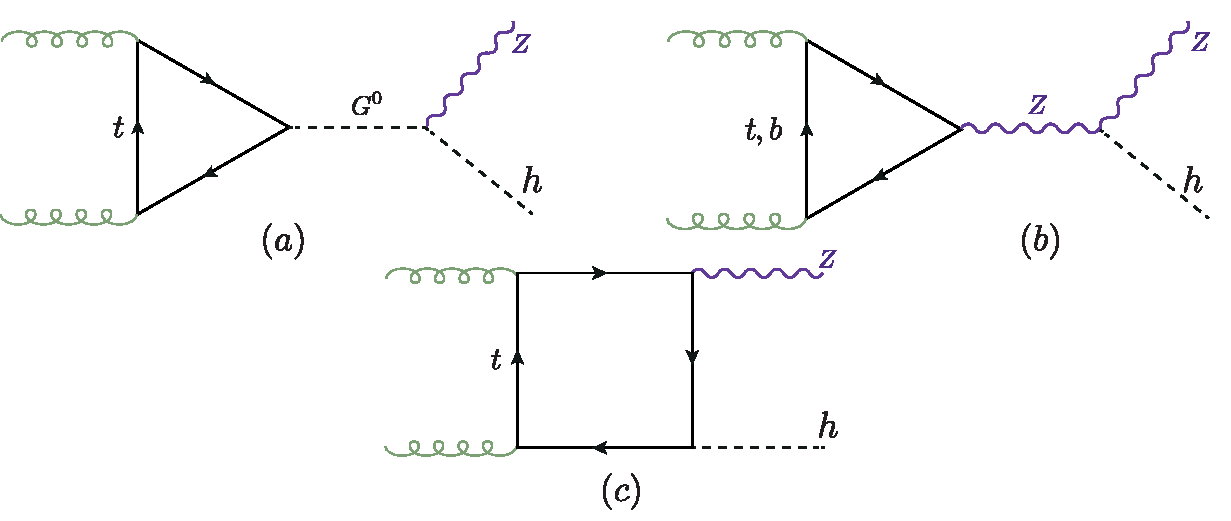
\includegraphics[width=12cm]{./figures/Feynman_LO}
		\caption{Example Feynman diagrams for the LO $gg \to Zh$ process. The triangle diagrams in a general $\xi$ gauge involve $Z$ and the neutral Goldstone~$G^0$ propagators. }
		\label{fig:dialo}
	\end{center}
\end{figure}
\par The LO ggF process has two sets of diagrams, the triangle, and the box, depicted in~\autoref{fig:dialo}. In (a), the triangle diagram contains a neutral Goldstone boson~$G^0$. Instead in (b), the $Z$ boson is mediated. The interplay between these two diagram types depends on the~$\xi$ gauge. Moreover, the $Z$ boson is strictly off-shell, due to Furry's theorem~\cite{PhysRev.51.125}.
In the Landau gauge, the $Z$-mediated diagrams will also vanish; this can be seen by considering the sub-amplitude~$ggZ^*$ that, in the Landau gauge, can be related to the decay of a massive vector boson
with mass $\sqrt{\hat{s}}$ into two massless ones. Such process is
forbidden by the Landau-Yang theorem \cite{Landau:1948kw, Yang:1950rg}. As a consequence, the triangle diagram can be obtained from the Goldstone-mediated one, which can be adopted from the results of pseudoscalar Higgs production~\cite{Spira:1995rr,Aglietti:2006tp}. 
The triangle diagrams are also proportional to the mass difference between the up- and down-type quarks. In this calculation, only the top quark is considered massive. Therefore, light quarks loops do not contribute to this process.

% It should be noted that triangle diagrams with $b$-quark loops contribute to $ \sim 1\%$ of the total amplitude, computed in the massless limit, i.e. $m_b \to 0$.  
%%%%%%%
\subsection{The transverse momentum expansion}
\label{sec:ptexp}
\par Choosing to expand in small $\pt$ of the $Z$ boson, the first step is expressing the transverse momentum in terms of the Mandelstam variables and masses 
\beq
\pt^2=\frac{\hat{t}\hat{u}-\mz^2\mh^2}{\hat{s}}.
\label{ptdef}
\eeq
From  eq.(\ref{ptdef}), together with the relation between
the Mandelstam variables, one finds 
\beq
\pt^2+\frac{\mh^2+\mz^2}{2}\leq\frac{\hat{s}}{4}+\frac{\dm^2}{\hat{s}},
\label{ptexp}
\eeq
where
$\dm = (\mh^2 -\mz^2)/2$. Eq.(\ref{ptexp}) implies 
$\pt^2/\hat{s} < 1$ that, together with the kinematical constraints
$\mh^2/\hat{s}< 1$ and
$\mz^2/\hat{s} < 1$. With these relations in mind, one can expand the amplitudes in terms of small  $\pt^2/\hat s$, $\mh^2/\hat{s}$ and $\mz^2/\hat{s}$, which is technically valid throughout the whole phase space, contrary to the HTL and HE limits.  The caveat for this expansion is that the amplitude does not depend on $\pt$ explicitly. Instead, one would expand in the reduced Mandelstam variables~$t^\prime/s^\prime\ll 1$ or $u^\prime/s^\prime\ll 1$, defined as
\beq
s^\prime=p_1\cdot p_2=\frac{\hat{s}}{2},~~
t^\prime=p_1\cdot p_3=\frac{\hat{t}-\mz^2}{2},~~ u^\prime =
p_2\cdot p_3=\frac{\hat{u}-\mz^2}{2},
\eeq
that satisfy
\beq
s^\prime + t^\prime + u^\prime =\dm.
\eeq
The choice of the expansion parameter~$t^\prime$ or ~$u^\prime$  depends on whether one expands in the forward or backwards kinematics. Because the process $gg \to Zh$ has two particles in the final states with different masses, the amplitude is not symmetric under their exchange.  Therefore, it is not possible to simply compute the cross-section via integrating the forward-expanded amplitude, contrary to what has been done for the Higgs pair production~\cite{Bonciani:2018omm}. To overcome this issue, the amplitude can be split into symmetric and anti-symmetric parts with respect to the exchange $ t^\prime \leftrightarrow u^\prime$, constructing directly symmetric and anti-symmetric projectors. Then, one can expand the symmetric part in the forward kinematics, like the Higgs pair case. Regarding the anti-symmetric part, the antisymmetric factor is simply extracted by multiplying the form-factors by $1/(\hat{t}-\hat{u})$. Afterwards,  the expansion in the forward kinematics can be preformed then the result should be multiplied back by $(\hat{t}-\hat{u})$.

\par In order to implement the $\pt$-expansion at the Feynman-diagram level, we start by splitting the momenta into longitudinal and transverse components with respect to the beam direction. This can be done by introducing the auxiliary vector~\cite{Bonciani:2018omm}, 
\begin{align}
	r^\mu &= p_1^\mu +p_3^\mu,
\end{align}
that satisfies
\beq
r^2= \hat{t},~~ r\cdot p_1=\frac{\hat{t}-\mz^2}{2},~~
r\cdot p_2=-\frac{\hat{t}-\mh^2}{2},
\label{rsp}
\eeq
and hence can be also written as
\beq
r^\mu =-\frac{\hat{t}-\mh^2}{\hat{s}}p_1^\mu +
\frac{\hat{t}-\mz^2}{\hat{s}} p_2^\mu + r_\perp^\mu =
\frac{t^\prime}{s^\prime}\,(p_2^\mu -p_1^\mu) - \frac{\dm}{s^\prime} \, p_1^\mu +
r_\perp^\mu,
\label{rpp}
\eeq
where
\beq
r_\perp^2=-\pt^2.
\eeq
substituting the definition of~$\pt$ from eq.\eqref{ptdef} one obtains
\beq
t^\prime = -\frac{s^\prime}2 \left\{ 1 - \frac{\dm}{s^\prime} \pm
\sqrt{\left( 1 - \frac{\dm}{s^\prime} \right)^2 -
	2 \frac{\pt^2 + \mz^2}{s^\prime}} \right\}
\label{tpdef}
\eeq
implying that the expansion in
small $\pt$ (the minus sign case in eq.(\ref{tpdef})) can be realised
at the level of Feynman diagrams, by expanding the propagators
in terms of the vector $r^\mu$ around $r^\mu \sim 0$ or, equivalently,
$p_3^\mu \sim -p_1^\mu$, see eq.(\ref{rpp}). 
%%%%
\section{Born cross-section in the $\pt$-expansion }
\label{sec:LOPtExp}
 As a baseline test for the validity and convergence behaviour of the~$\pt$-expansion, this method is first applied to the LO amplitude, and consequently used to compute the Born Partonic cross-section. The results are then compared to the exact cross-section calculation found in~\cite{Kniehl:1990iva, Dicus:1988yh}. \\ We start by defining the one-loop functions appearing in the similar calculation of the Born cross-section for ~$gg \to hh$ in the same expansion carried out in ref.~\cite{Bonciani:2018omm}
\bea
B_0[\hat{s},\mt^2,\mt^2] \equiv  B_0^+, &
B_0[- \hat{s},\mt^2,\mt^2]  \equiv B_0^- , &\\
C_0[0,0,\hat{s},\mt^2,\mt^2,\mt^2]  \equiv  C_0^+  ,& ~~~
C_0[0,0,-\hat{s},\mt^2,\mt^2,\mt^2]  \equiv C_0^- &
\eea
\beq
B_0[q^2,m_1^2,m_2^2] = \frac1{i\pi^2}
\int \frac{d^n k}{\mu^{n-4}} \frac1{(k^2 -m_1^2)((k+q)^2-m_2^2)},
\label{Bzero}
\eeq
\begin{align}
	%	\specialcell
	{ C_0[q_a^2,q_b^2,(q_a+q_b)^2, m_1^2,m_2^2,m_3^2] = \hfill }\nn  \\
	\frac1{i\pi^2}  \int \frac{d^d k}{\mu^{d-4}} \frac1{[k^2 -m_1^2][(k+q_a)^2-m_2^2]
		[(k-q_b)^2 - m_3^2]} &
	\label{Czero}
\end{align}
are the Passarino-Veltman functions \cite{Passarino:1978jh}, $d$ is the spacetime dimension and $\mu$ the 't Hooft mass.
%
 The $A_2$ and $A_6$ form-factors are given in~\autoref{cddorapp:due-oneloop}, as an example of symmetric and anti-symmetric form-factors. These form-factors are divided into triangle ($\triangle$) and
box ($\square$) contributions, and $B_0$ functions are understood as the
finite part of the integrals on the right hand side of eq.\eqref{Bzero}.
\par Using several truncations of the $\pt$-expansion, and comparing it to the exact LO result, one can see in~\autoref{fig:LO} the exact Born partonic LO cross-section (red line) as a function of the invariant mass of the $Zh$ system~$M_{Zh}$, in comparison to the $\pt$-expansions. 
For the numerical evaluation of the cross-section here and in
the following section, the SM input parameters are used 
\begin{equation}
	\begin{split}
		\mz=91.1876 \,\gev, ~~\mh=125.1 \gev, ~~  \mt=173.21\, \gev, \nn\\
		m_b = 0 \, \gev, ~~G_F= 1.16637\,\gev^{-2},~~ \alpha_s(\mz)=0.118.
	\end{split}
\end{equation}
From the ratio plotted in the lower panel of~\autoref{fig:LO}, we observe that the~$\mathcal{O}(\pt^0)$ expansion is in good agreement with the exact result when $M_{Zh}\lesssim 2\mt$. Inclusion of higher-order terms up to~$\mathcal{O}(\pt^6)$ extended the validity of the expansion to reach~$M_{Zh}\lesssim 750\gev$. This is the similar to what has been seen in~\cite{Bonciani:2018omm} for the Higgs pair production. Therefore, one would expect the $\pt$-expanded two-loop virtual correction to be an accurate approximation with the exact (numerical) result for the region of the invariant mass of  $M_{Zh}\sim 700-750\gev$. 
Similar conclusions can be derived from~\autoref{tab:partonic}, where it is shown that the partonic cross-section
expanded to order $\mathcal{O}(\pt^4)$ agrees with the full result for
$M_{ZH} \lesssim 600 \gev$  on the per-mille level.
The agreement further improves when $\mathcal{O}(\pt^6)$ terms are included.
\begin{table}
	\renewcommand{\arraystretch}{1.2}
	\centering
	\begin{tabular}{| c| c | c | c| c| c|} \hline
		\rowcolor{lightgray}  $M_{Zh}$ [GeV]  & $\mathcal{O}(\pt^0)$ & $\mathcal{O}(\pt^2)$ & $\mathcal{O}(\pt^4)$ & $\mathcal{O}(\pt^6)$ & full \\ \hline 
		\cellcolor{lightgray} 300 & 0.3547 & 0.3393 &  0.3373 &0.3371& 0.3371 \\
		\cellcolor{lightgray} 350 & 1.9385 & 1.8413& 1.8292 &1.8279& 1.8278 \\
		\cellcolor{lightgray} 400 & 1.6990 & 1.5347 & 1.5161 &1.5143& 1.5142 \\
		\cellcolor{lightgray} 600 & 0.8328 & 0.5653 & 0.5804 &0.5792&  0.5794 \\ 
		\cellcolor{lightgray} 750 & 0.5129 & 0.2482 & 0.3129 & 0.2841 &  0.2919 \\ \hline
	\end{tabular}
	\caption{The partonic cross-section $\hat{\sigma}^{(0)}$ at
		various orders in $\pt$ and the full computation for several values of~$M_{Zh}$, This table has been published in~\cite{Alasfar:2021ppe}. \label{tab:partonic}}
\end{table}
\begin{figure}[htpb!]
	\centering
	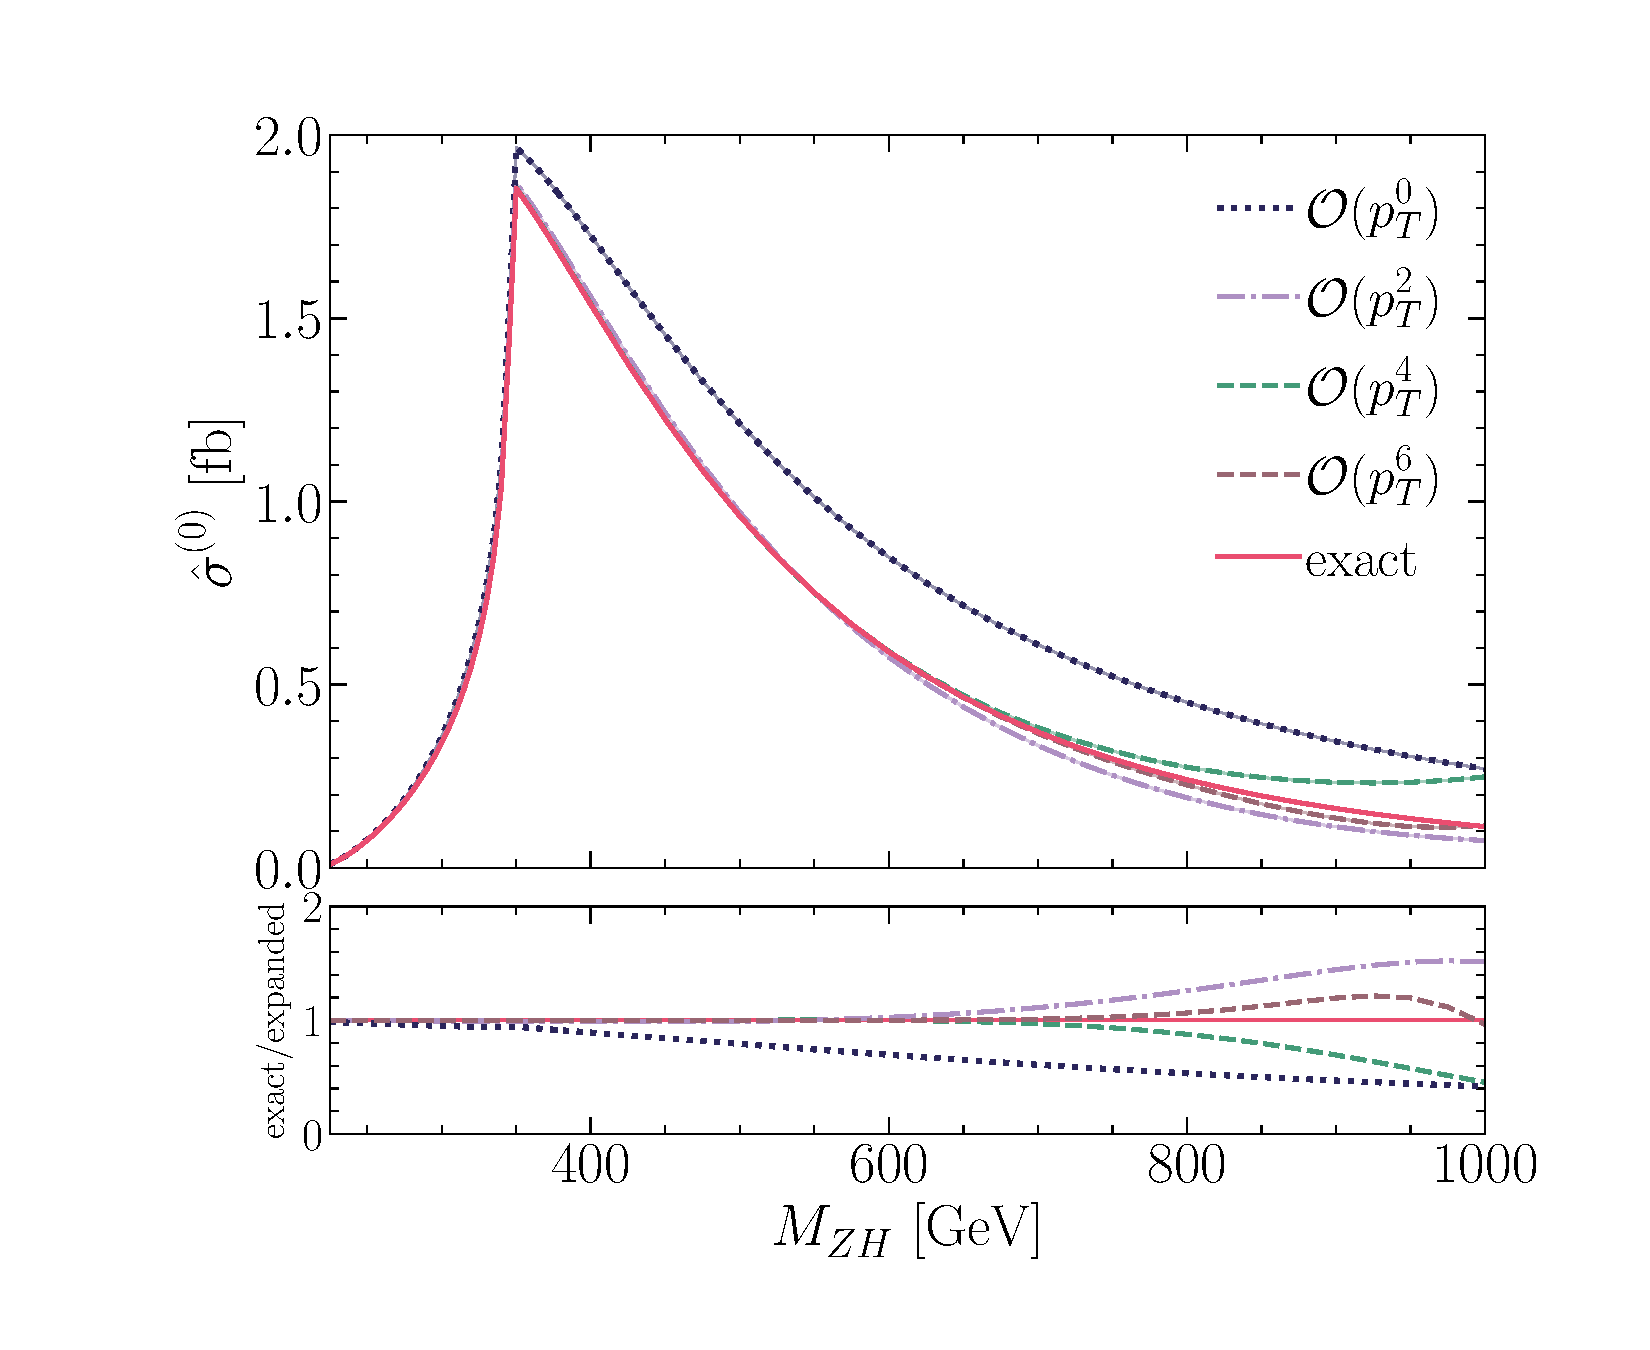
\includegraphics[width=0.75\linewidth]{./figures/LO_ptexp_ratio_1000.pdf}
	\caption{The Born partonic cross-section
		as a function of the invariant mass $M_{Zh}$.
		The exact result (red line) is plotted together with expansions at
		different orders in $\pt$ (dashed lines). In the bottom part,
		the ratios of the full result over the $\pt$-expanded ones at
		various orders are shown. This plot has been published in~\cite{Alasfar:2021ppe}.}
	\label{fig:LO}
\end{figure}
%%%%%%%
\section{ NLO calculation }
\label{sec:quattro}
\autoref{fig:dianlo} shows example Feynman diagrams for the virtual two-loop corrections to $gg \to Zh$, which involve corrections to the triangle topology in (a) and (b), corrections to the box topology in (c); also (d) shows a new topology a double triangle. Both two-loop corrections to the triangles and the double triangle diagrams can be computed analytically. The loop-integrals of the triangle contributions effectively depend on one scale only, while the double-triangles' are products of two one-loop integrals. The boxes are much more difficult as they depend on several mass scales. This makes the reduction to MI's extremely challenging. Moreover, even if that were possible, not all of the MI's will have been analytically solved thus far.
\begin{figure}[htpb!]
	\begin{center}
		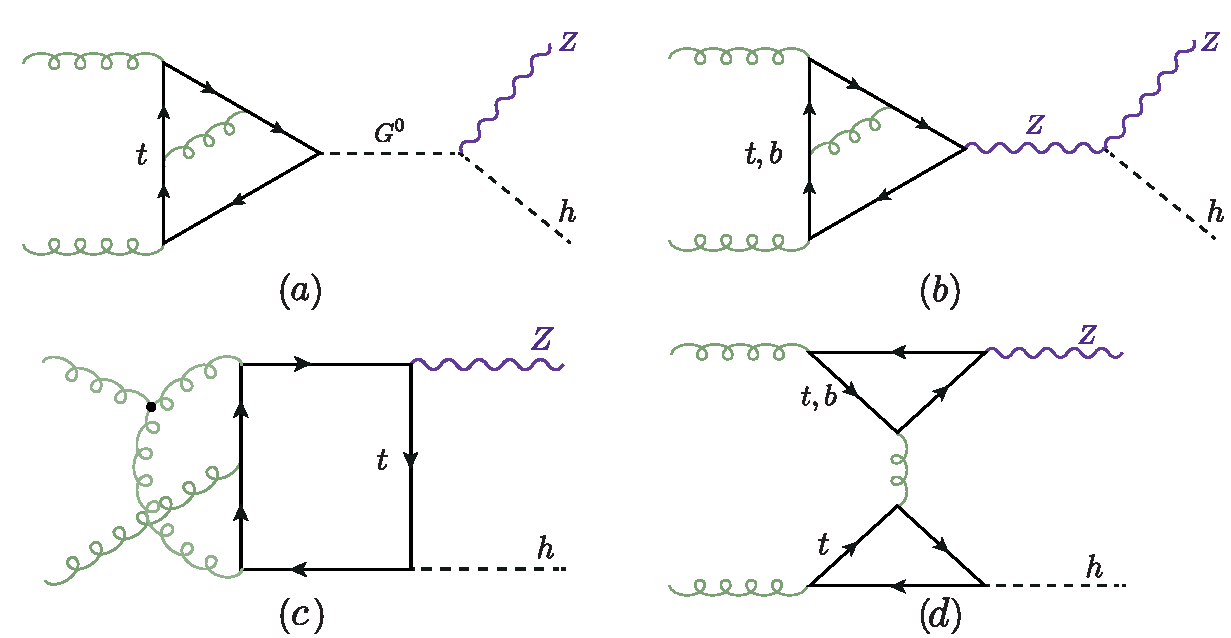
\includegraphics[width=12cm]{./figures/Feynman_NL0}
		\caption{Feynman diagrams examples for the virtual NLO corrections to the $gg \to Zh$ process. }
		\label{fig:dianlo}
	\end{center}
\end{figure}
\subsection{Renormalisation}
\label{subsec:ren}
The two-loop corrections to the triangle and box diagrams contain both UV and IR divergences. The first emerges from UV divergent sub-diagrams, such as top-quark mass renormalisation and QCD vertex correction, while the lR divergences come from massless loops. In order to remove these divergences, are needed. Instead, the double triangle topology is both UV and IR finite.
%\par The gluon wavefunction renormalisation of the incoming gluons (external legs) is achieved by multiplying the amplitude by the renormalisation factor~$ Z_A^{1/2}$ for each gluon.
%\begin{equation}
%	Z_A= 1+\as \frac{2}{3\epsilon} \left( \frac{\mu_R^2}{m_t^2} \right) ^\epsilon.
%\end{equation}
The on-shell scheme for the top-quark mass renormalisation has been used, in which the bare mass is replaced by the renormalised one~$ m_0 = Z_m m$  in the propagators. This gives the $\MSbar$ renormalised mass. 
%This can be done by multiplying $ \delta Z_m$ with the derivative of the one-loop form-factor with respect to the  mass., here $Z_m$ is given by
\begin{equation}
	Z_m = 1+ C_F \frac{3}{\epsilon}.
\end{equation}
In order to convert the mass definition to the on-shell scheme, it is possible to add the finite renormalisation term
\begin{equation}
	Z^{OS}_m = 1- 2 C_F,
\end{equation}
here $C_F=(N_c^2-1)/2N_c$ is one of the two Casimir invariants of QCD along with~$ C_A=N_c$. 
The $q \bar q g$ vertex correction involves a renormalisation of the strong couplings constant $ \alpha_s$, which is achieved via replacing the bare constant $\alpha_s^0$ with the renormalised one, hence it becomes  $ \alpha^0_s = \frac{\mu_R^{2\epsilon}}{S_\epsilon}  \Zas \alpha_s$, where
\begin{equation}
	\Zas = 1- \frac{\alpha_s}{4 \pi} \, \frac{1}{ \epsilon}\,  \left( \beta_0-\frac{2}{3} \right) \left(\frac{\mu_R^2}{m_t^2} \right) ^\epsilon,
\end{equation}
and the constant $ \beta_0 = \frac{11}{3} C_A -\frac{2}{3}N_f$, where $N_f$ is the number of ``active'' flavours. The 5-flavour scheme $N_f=5$ is adopted here.  This is only done for the triangle diagrams, as for the boxes the background field gauge was used, which renders the renormalisation of $\alpha_s$ unnecessary. 
\par The loop integrals were evaluated using dimensional regularisation in $d= 4-2\epsilon$ dimensions. This scheme requires some caution when $\gamma_5$ is present in the amplitude. The approach followed in this calculation is letting $\gamma_5$ naively anti-commute with all $d$-dimensional $\gamma_\mu$'s, and then correct that with the finite renormalisation constant known as \textbf{Larin counter-term}~\cite{Larin:1993tq}
\begin{equation}
	Z_5 = 1- 2\, C_F.
\end{equation}
The renormalised amplitude is written as
\begin{equation}
	\mathcal M  (\alpha_s, m, \mu_R) = Z_A \mathcal M( \alpha_s^0, m^0).
\end{equation}
Putting all the above substitutions together, we get the renormalised two-loop form-factor:
\begin{align}
	( \mathcal A ^{(1)})^R &= 	\mathcal A ^{(1)} -	\mathcal A_{UV} ^{(0)}- 	\mathcal A_{UV, m} ^{(0)} + \mathcal A_{\text{Larin}} ^{(0)}   \\
	\mathcal A_{UV} ^{(0)} &= \asr\,\frac{\beta_0}{\epsilon} \left( \frac{\mu_R^2}{\hat s} \right) ^{ -\epsilon} 	\mathcal A ^{(0)}.  \nonumber \\
	\mathcal A_{UV, m} ^{(0)} &= \asr \, \left( \frac{3}{\epsilon} -2\right) C_F \left( \frac{\mu_R^2}{\hat s} \right) ^{ -\epsilon} m^0 \partial_m \mathcal A^{(0)} . \nonumber \\
	\\
	\mathcal	A_{\text{Larin}} ^{(0)}  &= - \asr \, C_F  \mathcal A ^{(0)} .\nonumber
\end{align}
The following IR-counter-term is used in order to cancel the IR divergences
\begin{equation}
	\mathcal A_{IR} ^{(0)}  = \frac{e^{\gamma_E \epsilon}}{\Gamma(1-\epsilon)} \, \asr \left( \frac{\beta_0}{\epsilon} + \frac{ C_A}{\epsilon^2} \right)  \, \left(  \frac{\mu_R^2}{\hat s}\right) ^{2\epsilon} \mathcal A ^{(0)}.
\end{equation}
The one-loop form-factors, need to be expanded up to order $ \mathcal O(\epsilon^2) $, for the UV and IR counter-terms.
%%%%%
\subsection{Calculation of the exact virtual corrections}
The two-loop calculations of the triangle digrams involves the diagrams with $Z^*$ and $G^0$ propagators, depending on the gauge of choice. Observations found in ref.~\cite{Altenkamp:2012sx} shows that due to Landau-Yang theorem in the Landau gauge, all diagrams with the  $Z^*$ exchange vanish. Therefore, the part of the top triangle diagrams  can be obtained from the decay amplitude of a pseudoscalar boson into two gluons that is known in the literature in the full mass dependence up to NLO terms~\cite{Spira:1995rr,Aglietti:2006tp}. On the contrary, using the unitary gauge, the NLO calculation needs to be done with the $Z^*$ exchange diagrams only.  The calculations in these two gauges result in apparently different Lorentz structures that are linked via the Schouten identity 
\begin{equation}
	q^\alpha \epsilon^{\beta \gamma \delta  \phi} + q^\beta \epsilon^{\gamma \delta  \phi \alpha}+ q^\gamma \epsilon^{ \delta  \phi \alpha \beta} +q^\gamma \epsilon^{ \delta  \phi \alpha \beta} + q^\delta \epsilon^{   \phi \alpha \beta \gamma } +  q^\phi \epsilon^{ \alpha \beta \gamma \delta } =0 .
\end{equation}
A cross-check has been preformed in order to ensure that the NLO calculation introduces no new Lorentz structures, and gives the same result in a general $ R_\xi$ gauge as the results in~\cite{Spira:1995rr,Aglietti:2006tp}. The two-loop calculation has been carried out in the~$ R_\xi$ gauge. The amplitudes have been automatically generated by \texttt{FeynArts} \cite{Hahn:2000kx} and
contracted with the projectors as defined in \autoref{app:uno}
using \texttt{FeynCalc }\cite{Mertig:1990an,Shtabovenko:2016sxi} and \texttt{Package X}~\cite{Patel:2016fam} and in-house
Mathematica routines. The two-loop integrals were reduced to a set of master integrals~MI, illustrated graphically in~\autoref{fig:trimis} using \texttt{Kira}~\cite{Maierhofer:2017gsa}.
\begin{figure}[htpb!]
	\begin{center}
		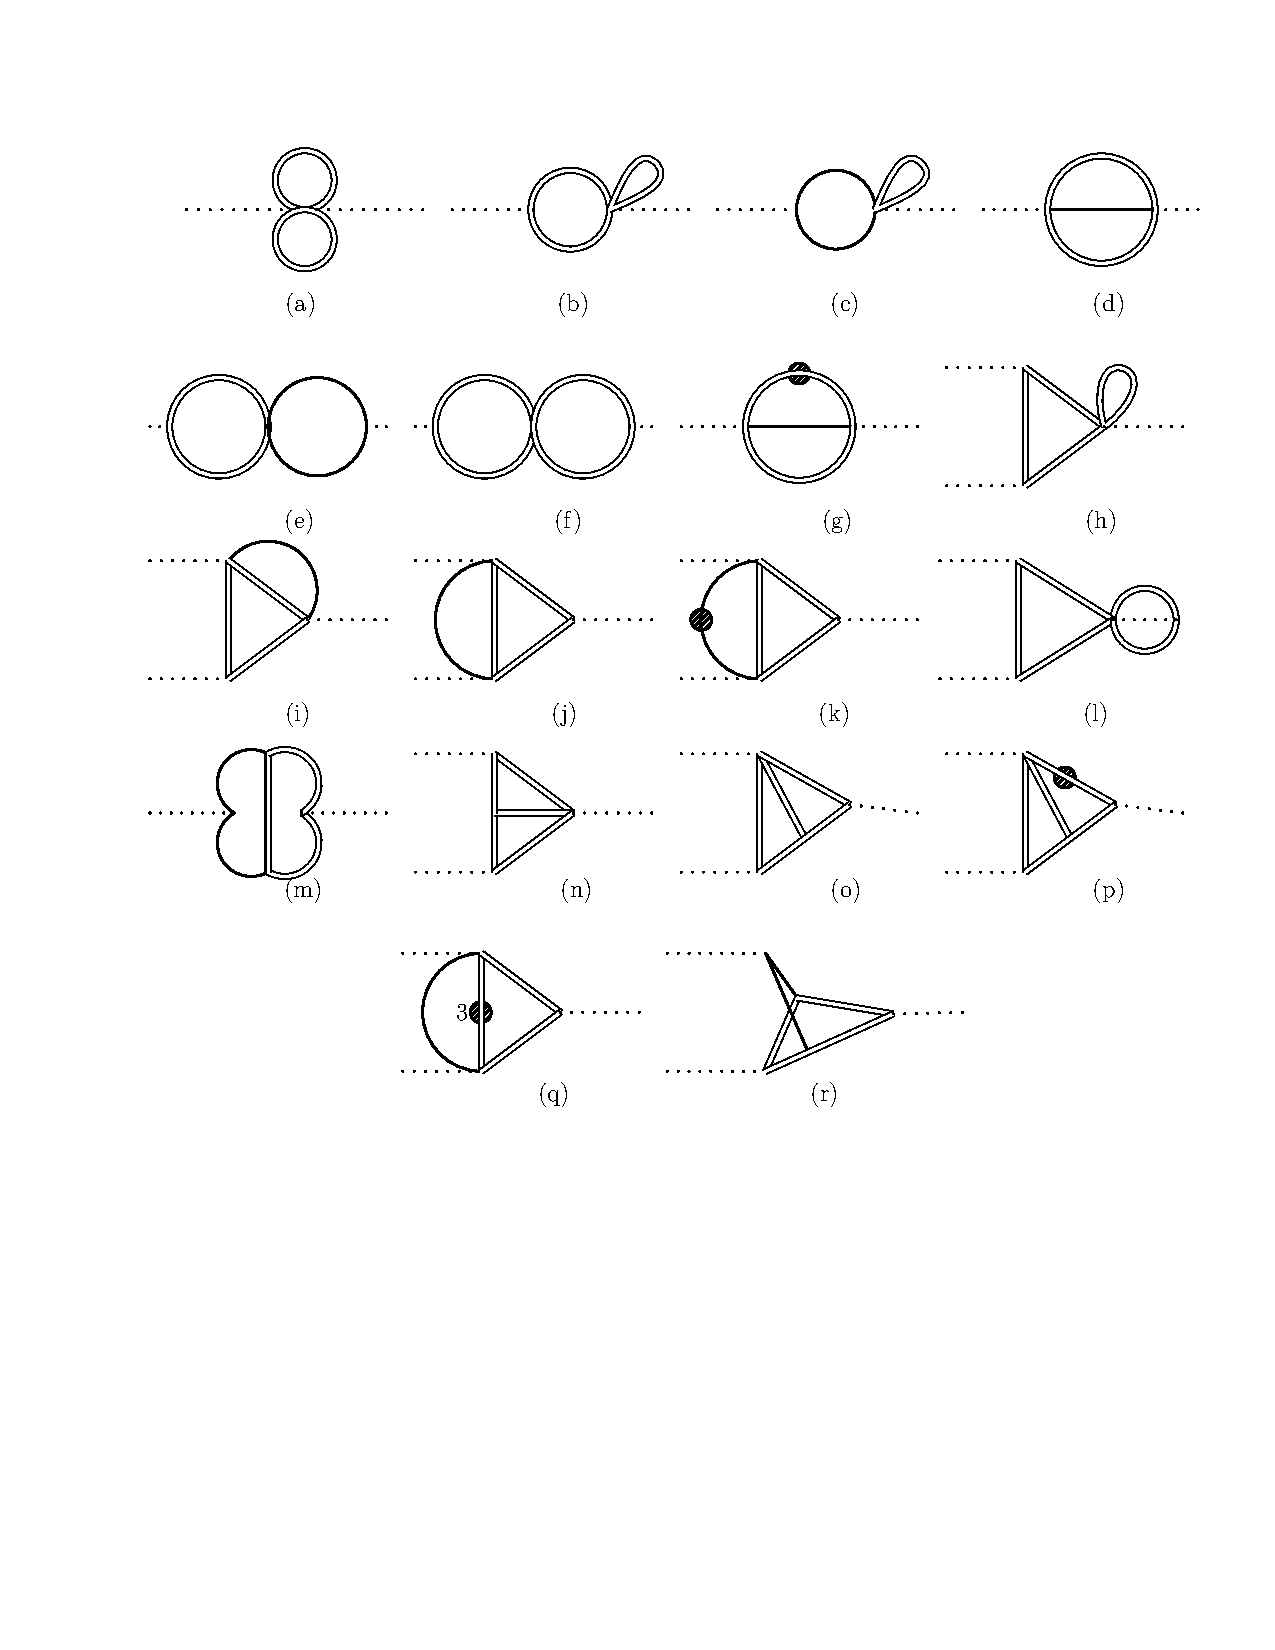
\includegraphics[width=12cm]{./figures/MI}
		\caption{ The list of two-loop master integrals (MI's) resulting from the reduction of the two-loop triangle corrections. The product of one-loop MI's appearing in this list also appear in the calculation of the double-triangle diagrams. A single line denotes a massless propagator, while a double line denotes a massive one. The dot denotes a squared propagator unless the number of the exponent is indicated.}
		\label{fig:trimis}
	\end{center}
\end{figure}
These MI's are either products of one-loop functions (a)-(c), (e),(f),(h) and (l) or can be found in the literature~\cite{Bonciani:2003hc,Aglietti:2006tp}. Their implementation in this calculation has been validated numerically using \texttt{SecDec}~\cite{Borowka:2013cma,Borowka:2015mxa}.  
The virtual correction for the triangle diagrams can be separated according to their colour factors into
\begin{equation}
	\mathcal A ^{(1)}   = C_F \mathcal A_{CF} ^{(1)}  + C_A \mathcal A_{CA} ^{(1)},
\end{equation}
The $C_A$ part contains a double pole $ \mathcal O( 1/\epsilon^2)$ and a single pole $ \mathcal O( 1/\epsilon)$. Whilst the $C_F$ part only contains a UV divergent single pole, which needs to be cancelled via mass and vertex renormalisation. The poles do not have a dependence on the renormalisation scale $ \mu_R$. However, there is a dependence on that scale in the finite part, as well.  No new Lorentz structures appears, and the final result in $R_\xi$ matched the one found in~\cite{Spira:1995rr,Aglietti:2006tp} for the Landau gauge. The explicit results are shown in~\autoref{app:due}
%
\par  The calculation of the double triangle diagrams (d) of~\autoref{fig:dianlo} is fairly straightforward, all of the 
integrals can be rewritten in terms of products of one-loop functions. All of the Lorentz structures appear in the double triangle except for~$\mathcal{P}_6$, analogous to the triangle case. The explicit forms of form-factors corresponding to these structures is presented in~\autoref{app:due}. Although in this calculation, the amplitude has been written using a different
tensorial structure compared to ref.\cite{Davies:2020drs}. It was  checked,
using the relations between the two tensorial structures reported in 
\autoref{app:uno} that the result obtained here is in agreement with the one presented
in ref.~\cite{Hasselhuhn:2016rqt}.
\subsection{Calculation of the $\pt$-expanded virtual corrections}
%%%
\par The two-loop triangle diagrams can also be interpreted as an expansion in $\pt$, but this expansion terminates at~${\cal O}(\pt^2)$, rather than being an infinite series. Hence, in this section, we concentrate on the two-loop box diagrams $\pt$-expansion~\footnote{The calculation of the box diagrams has been done by my collaborators, the co-authors of~\cite{Alasfar:2021ppe}.}.\\
%%%%
Like the two-loop triangle diagrams, the box diagrams amplitudes were generated and projected through the same pipeline. After the contraction of the epsilon tensors, the diagrams were expanded as
described in~\autoref{sec:ptexp}, keeping only ${\cal O}(\pt^4)$ terms. They were reduced to MI's
using \texttt{FIRE} \cite{Smirnov:2014hma} and \texttt{LiteRed} \cite{Lee:2013mka}. The
resulting MI's were identical to those for Higgs pair
production \cite{Bonciani:2018omm}. Nearly all of them are expressed
in terms of generalised harmonic polylogarithms, except for
two elliptic integrals \cite{vonManteuffel:2017hms, Bonciani:2018uvv}. The renormalisation and IR pole subtraction procedure was carried out as prescribed~\autoref{subsec:ren}. Furthermore, the treatment of $\gamma_5$ was cross-checked with a Pauli-Villar regulator in the HTL.\\
The two-loop box diagrams were also computed in the HTL up to  $\mathcal{O}(1/\mt^6)$. These results were confronted with the $\pt$-expanded are after expanding them in small $\hat s/m_t^2$, providing a cross-check of the expansion. 
%%%%%
\section{Results and conclusions} \label{sec:hzres}
The virtual corrections to the ggF $Zh$ production have been implemented in a  \texttt{FORTRAN} code using  \texttt{handyG}~\cite{Naterop:2019xaf}, for the evaluation of generalised harmonic polylogarithms and \texttt{Chaplin}~\cite{Buehler:2011ev} for the harmonic polylogarithms appearing in the triangle two-loop functions. 
On the other hand, the elliptic integrals are evaluated using the routines developed in
ref.~\cite{Bonciani:2018uvv}. Since the result is analytic, the code is significantly faster than the numerical evaluation of the two-loop amplitude~\cite{Chen:2020gae}, with evaluation time of ca. 0.1 sec per one phase space point on a personal laptop.\\
In order to facilitate the comparison of these results with the ones
presented in the literature, we define the finite part of the virtual corrections
as in
ref.\cite{Davies:2020drs}\footnote{The definition of the matrix elements here
	differs by a factor of
	$\frac{1}{\hat{s}}$ from ref.~\cite{Davies:2020drs}, \textit{cf}. also
	\autoref{app:uno}.}
\begin{equation}
	\begin{split}
		\mathcal{V}_{fin}&=\frac{G_F^2 m_Z^2}{16}\left(\frac{\alpha_s}{\pi}\right)^2
		\left[ \sum_{i} \left|\mathcal{A}_i^{(0)} \right|^2\frac{C_A}{2}\left(\pi^2-
		\log^2\left(\frac{\mu_R^2}{\hat{s}}\right)\right)\right. \\
		& \left. +2\sum_i\text{Re}\left[\mathcal{A}_i^{(0)}\left(\mathcal{A}_i^{(1)}\right)^*\right]\right] ,
		\label{eq:vfin}
	\end{split}
\end{equation}
and in the numerical evaluation of eq.(\ref{eq:vfin}) is fixed
$\mu_R= \sqrt{\hat{s}}$.
The triangle and HTL box topologies were validated against the results of refs.~\cite{Hasselhuhn:2016rqt,Davies:2020drs} finding perfect
agreement at the form-factor level, i,.e.~$\mathcal{A}_i^{(1)}$. \\

The finite virtual part of the partonic cross-section in eq.~\eqref{eq:vfin} is defined  by
\begin{equation}
	\Delta \hat{\sigma}_{virt}=
	\int_{\hat{t}^-}^{\hat{t}^+} d\hat{t}
	\frac{\alpha_s}{16\pi^2}\frac{1}{\hat{s}^2}\mathcal{V}_{fin}\, .
	\label{eq:deltasigma}
\end{equation}
This function is used to compare the $\pt$-expanded results with the other expansion methods. Starting with low $M_{Zh}$, 
the $\pt$-expanded is compared with the HTL~$\mathcal{V}_{fin}$, finding an excellent numerical agreement.
It is important to note that, at the same order in the expansion, 
the $\pt$-expanded terms are more accurate than
the HTL ones, albeit computationally more demanding.  Additional checks have been done using the numerical evaluation of the NLO amplitude by~\cite{Chen:2020gae}, where the authors have evaluated the exact two-loop MI's using \texttt{pySecDec}~\cite{Borowka:2017idc, Borowka:2018goh}.  \autoref{tab:comparison} shows a comparison between the $\pt$-expanded~$\mathcal{V}_{fin} 4/(\as^2 \alpha^2)$ vs the exact numerical result of~\cite{Chen:2020gae} for several phase space points. 
As can be seen from the table the relative difference 
between the two results is less than half a per-mille.
\begin{table}
	\renewcommand{\arraystretch}{1.2}
	\centering
	\begin{tabular}{| c| c | c | c| } \hline
		\rowcolor{lightgray}  $\hat{s}/m_t^2$ & $\hat{t}/m_t^2$ &  ref.\cite{Chen:2020gae} & $\mathcal{O}(\pt^6)$  \\ \hline 
		\cellcolor{lightgray} 1.707133657190554 & \cellcolor{lightgray} -0.441203767016323 & 35.429092(6) & 35.430479 \\
		\cellcolor{lightgray} 3.876056604162662 & \cellcolor{lightgray} -1.616287256345735 & 4339.045(1) & 4340.754 \\
		\cellcolor{lightgray} 4.130574250302561 & \cellcolor{lightgray} -1.750372271104745 & 6912.361(3) & 6915.797 \\
		\cellcolor{lightgray} 4.130574250302561 & \cellcolor{lightgray} -2.595461551488002 & 6981.09(2) & 6984.20  \\ \hline
	\end{tabular}
	\caption{Comparison of $\mathcal{V}_{fin} 4/(\alpha_s^2 \alpha^2)$ with the numerical results of ref.~\cite{Chen:2020gae}. This table has been published in~\cite{Alasfar:2021ppe}. \label{tab:comparison}}
\end{table}
\begin{figure}[th]
	\centering
	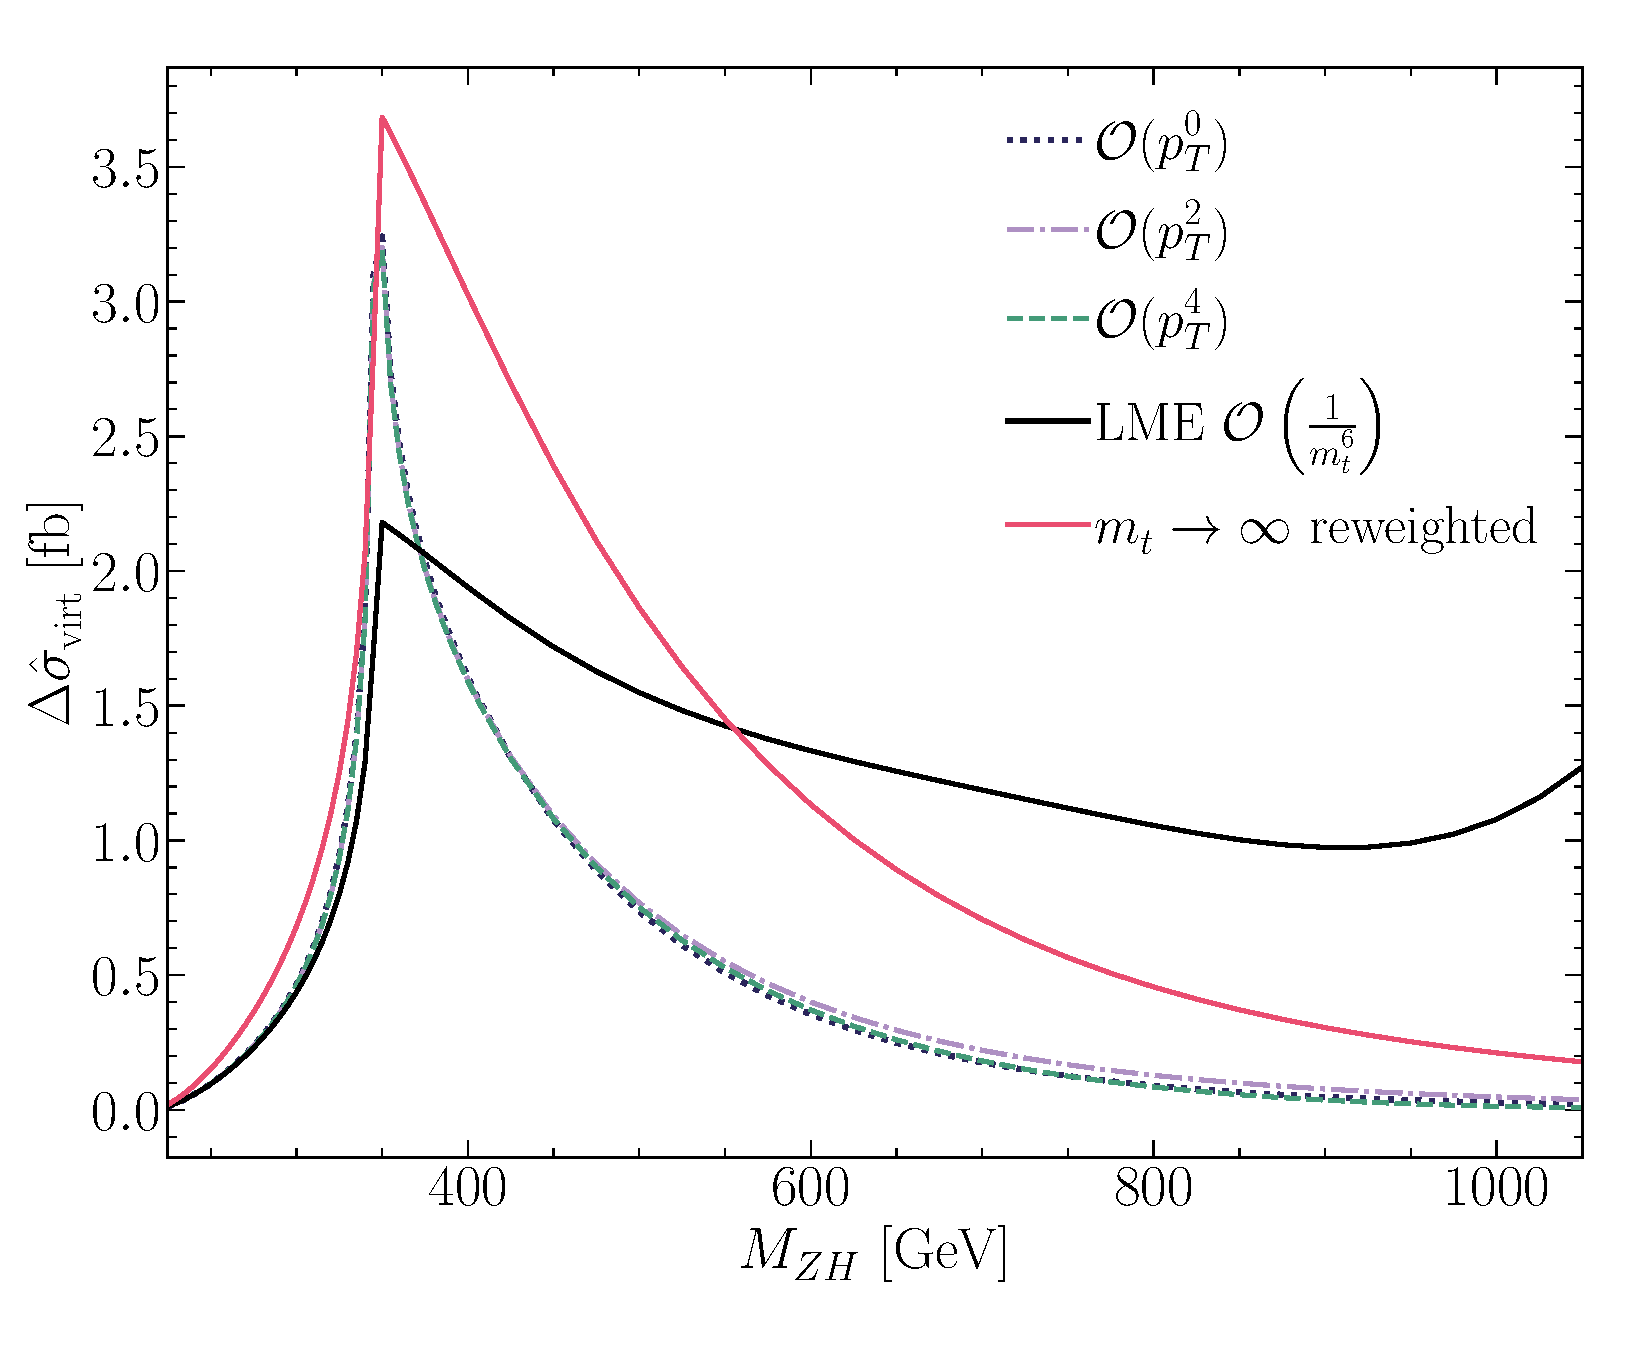
\includegraphics[width=0.7\textwidth]{./figures/sigma_part_virt_LMEreweighted.pdf}
	\caption{$\Delta \hat{\sigma}_{virt}$ defined by eq.\eqref{eq:deltasigma}, shown as a function of $M_{Zh}$. The various orders of the $\pt$-expansion are plotted as dashed lines, while the black and red continuous lines stand for the HTL and reweighted $m_t \rightarrow \infty$ results, respectively.This plot has been published in~\cite{Alasfar:2021ppe}.}
	\label{fig:deltasigma}
\end{figure}
%%%%%%%%%%

In \autoref{fig:deltasigma}, the dashed lines show
the different orders of the expansion in $\pt$. 
For all parts of the matrix elements, the best results
available were used. The triangle and double-triangle
topologies were evaluated exactly, while the boxes various orders in the $\pt$-expansion were used.
For comparison, the results are shown where
$\mathcal{A}^{(1)}$ is replaced by the one computed in HTL up to
$\mathcal{O}(1/m_t^6)$ (full black line), which, is valid
up to $M_{Zh}< 2 \mt$.  Within the validity of the HTL, the $pt$-expanded
results agree well with it.
Furthermore, the results in the infinite top
mass limit reweighted by the full amplitudes squared can be seen as the full red line in the plot, corresponding to the approach of ref.\cite{Altenkamp:2012sx}, keeping though the double triangle
contribution in full top mass dependence. 
Differently from the HTL line, the $\mt \to \infty$ reweighted one
shows a behaviour, for  $M_{Zh} \gtrsim 400\gev$, similar to the behaviour of
the $\pt$ lines. Still,   the difference
between the reweighted result and the $\pt$-expanded ones is significant.
The $\pt$-expanded results show
very good convergence.  The zero-order in term of the $\pt$- expansion agrees
exceptionally well with the higher orders, and all the
three results are very close up to $M_{Zh} \sim 500\gev$.
%%%%%%%%%%%%%%%%%%%%%%%%%%%%%%%
\par In conclusion, we have shown that the $\pt$-expansion can be applied to a very good accuracy to $gg\to Zh$.  The same MI's that were found for Higgs pair production \cite{Bonciani:2018omm} also appear in the $Zh$ virtual corrections. Predominantly, these MI's are expressed in terms of generalised harmonic polylogarithms except two elliptic integrals. Using the LO calculation, we have shown the validity of the $\pt$-expansion covering the invariant mass interval  $M_{Zh}\lesssim 750\text{ GeV}$, which covers $\sim 98\%$ of the total phase space for~$13-14$ TeV energies.\\
The $\pt$-expansion agrees within per mill level accuracy with the numerical results found in~\cite{Chen:2020gae}. However, it allows for fast amplitude computation with less than $0.1$ second per phase space point using a modern laptop with mid-range specifications. Furthermore, the integration over the $\hat{t}$ variable
in eq.(\ref{eq:deltasigma}) converges superbly.  With the flexibility of these analytic
results, an application to the beyond-the SM is certainly
possible.\\ 
Finally, it should be noted that this calculation complements
nicely the results obtained in ref.~\cite{Davies:2020drs} using a HE
expansion, which according to the authors, provides precise results for
$\pt \gtrsim 200\gev$. The merging of the two analyses provided
a result that covers the whole phase space, and can be easily implemented into a
Monte Carlo code. A combination of the two expansions for the virtual corrections has been published in~\cite{Bellafronte:2022jmo}.